\documentclass[11pt]{article}
\usepackage{amsmath}
\usepackage{amssymb}
\usepackage{graphicx}
\usepackage{fancyhdr}
\usepackage{enumerate}
\usepackage{titlesec}
\usepackage[colorlinks=true,urlcolor=blue]{hyperref}
\usepackage{subcaption}

\titlespacing{\subsubsection}{0pt}{0pt}{0pt}

% No page numbers
%\pagenumbering{gobble}

% INFORMATION SHEET (DO NOT EDIT THIS PART) ---------------------------------------------
\newcommand{\addinformationsheet}{
\clearpage
\thispagestyle{empty}
\begin{center}
\LARGE{\bf \textsf{Information sheet\\CS224W: Social and Information Network Analysis}} \\*[4ex]
\end{center}
\vfill
\textbf{Assignment Submission } Fill in and include this information sheet with each of your assignments.  This page should be the last page of your submission.  Assignments are due at 11:59pm and are always due on a Thursday.  All students (SCPD and non-SCPD) must submit their homeworks via GradeScope (\url{http://www.gradescope.com}). Students can typeset or scan their homeworks. Make sure that you answer each (sub-)question on a separate page. That is, one answer per page regardless of the answer length. Students also need to upload their code at \url{http://snap.stanford.edu/submit}. Put all the code for a single question into a single file and upload it. Please do not put any code in your GradeScope submissions. 
\\
\\
\textbf{Late Homework Policy } Each student will have a total of {\em two} free late periods. {\em Homeworks are due on Thursdays at 11:59pm PDT and one late period expires on the following Monday at 11:59pm PDT}.  Only one late period may be used for an assignment.  Any homework received after 11:59pm PDT on the Monday following the homework due date will receive no credit.  Once these late periods are exhausted, any assignments turned in late will receive no credit.
\\
\\
\textbf{Honor Code } We strongly encourage students to form study groups. Students may discuss and work on homework problems in groups. However, each student must write down their solutions independently i.e., each student must understand the solution well enough in order to reconstruct it by him/herself.  Students should clearly mention the names of all the other students who were part of their discussion group. Using code or solutions obtained from the web (github/google/previous year solutions etc.) is considered an honor code violation. We check all the submissions for plagiarism. We take the honor code very seriously and expect students to do the same. 
\vfill
\vfill
}
% ------------------------------------------------------------------------------

% MARGINS (DO NOT EDIT) ---------------------------------------------
\oddsidemargin  0.25in \evensidemargin 0.25in \topmargin -0.5in
\headheight 0in \headsep 0.1in
\textwidth  6.5in \textheight 9in
\parskip 1.25ex  \parindent 0ex \footskip 20pt
% ---------------------------------------------------------------------------------

% HEADER (DO NOT EDIT) -----------------------------------------------
\newcommand{\problemnumber}{0}
\newcommand{\myname}{name}
\newfont{\myfont}{cmssbx10 scaled 1000}
\pagestyle{fancy}
\fancyhead{}
\fancyhead[L]{\myfont Question \problemnumber, Problem Set 1, CS224W}
%\fancyhead[R]{\bssnine \myname}
\newcommand{\newquestion}[1]{
\clearpage % page break and flush floats
\renewcommand{\problemnumber}{#1} % set problem number for header
\phantom{}  % Put something on the page so it shows
}
% ---------------------------------------------------------------------------------


% BEGIN HOMEWORK HERE
\begin{document}

% Question 1.1
\newquestion{1.1}

The degree distribution of the two random graphs both show a peak at around the degree of 8, and then decay quickly to nearly zero. While the degree distribution of the real-world network decays from the very beginning but it decays at a slower speed than the random ones'. It also shows some fluctuation at the region of higher degree.

\begin{figure}
\centering
\begin{subfigure}{.55\textwidth}
  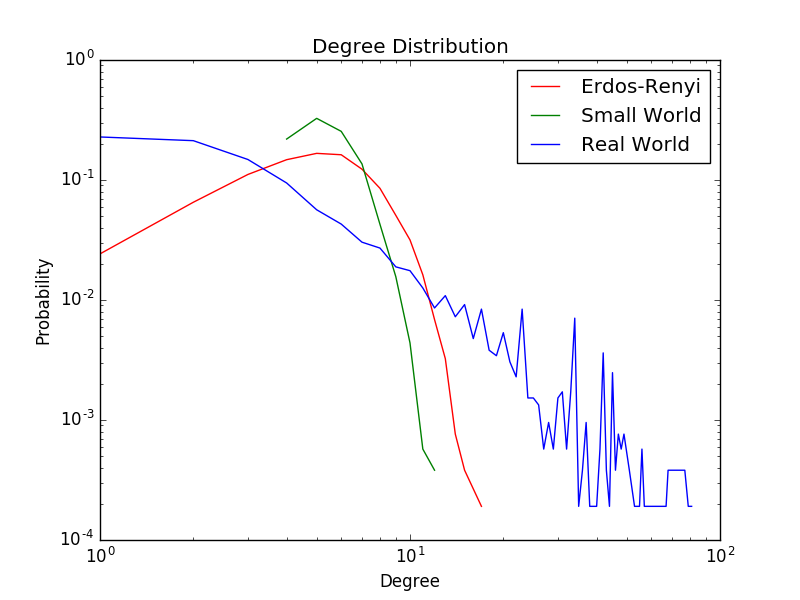
\includegraphics[width=\textwidth]{DegDist.png}
  \caption{Log-log degree distribution}
  \label{fig:Log-log degree distribution}
 \end{subfigure}
 \begin{subfigure}{.55\textwidth}
    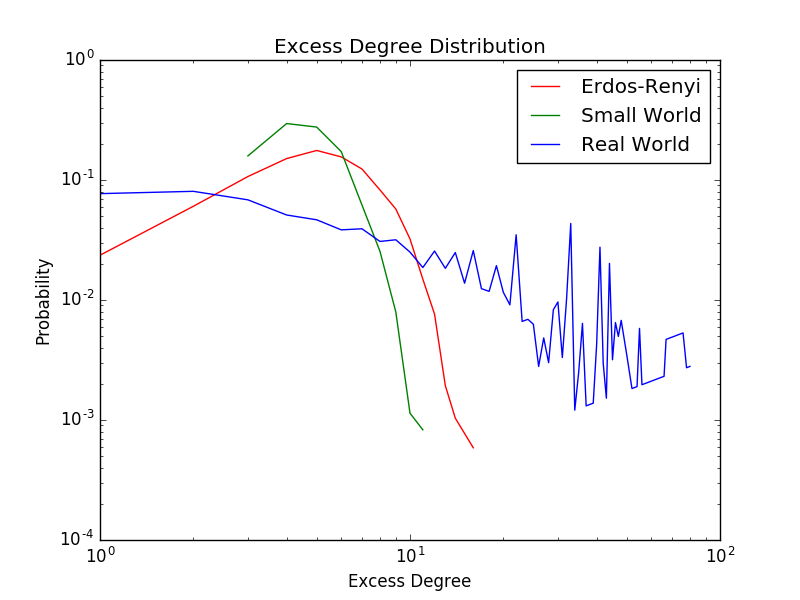
\includegraphics[width=\textwidth]{ExDegDist.png}
  \caption{Log-log excess degree distribution}
  \label{fig:Log-log excess degree distribution}
  \end{subfigure}
\end{figure}


% Question 1.2
\newquestion{1.2}

\subsubsection*{(a)}
Key difference:\\
The excess degree distribution of the real-world network decays much slower than its degree distribution.\\

The expected degrees:\\
Erdos-Renyi: 5.526\\
Small-World: 5.526\\
Real-World: 5.526\\
\\
The expected extra degrees:\\
Erdos-Renyi: 5.553\\
Small-World: 4.803\\
Real-World: 15.870\\
\\


\subsubsection*{(b)}
By the definition of $q_k'$ we can find out that it is in fact counting the number of nodes with degree $k+1$ and each of these nodes are counted $k+1$ times since they are connected to $k+1$ other nodes. Therefore, we have $q_k'=(k+1)p_{k+1}'$. Since $p_k'=Cp_k$ where $C=\sum_{i=1}^{n}p_i$ is a constant, we have that
\begin{align}
q_k&=\frac{q_k'}{\sum_{i=1}^{n}q_i'}\\
&=\frac{(k+1)p_{k+1}'}{\sum_{i=1}^{n}(i+1)p_{i+1}'}\\
&=\frac{(k+1)Cp_{k+1}}{\sum_{i=1}^{n}(i+1)Cp_{i+1}}\\
&==\frac{(k+1)p_{k+1}}{\sum_{i=1}^{n}(i+1)p_{i+1}}
\end{align}
The above is the fomula that we can use to calculate $q_k$ from $p_k$
% Question 1.3
\newquestion{1.3}
The average clustering coefficient:\\
Erdos-Renyi: 0.0018\\
Small-World: 0.1847\\
Real-World: 0.5296\\

The real-world network has the largest clustering coefficient.\\

Because the real-world is a collaboration network for scientific researchers. Two persons who have both collaborated with a third person in some papers have naturally very high probability of collaborating in a paper. Therefore the network has very high clustering coefficient.

% Question 2.1
\newquestion{2.1}
Davis, Mark (V)\\
Sanders, Alex (I)\\
North, Peter (I)\\
Marcus, Mr.\\
Tedeschi, Tony\\
Dough, Jon\\
Stone, Lee (II)\\
Voyeur, Vince\\
Lawrence, Joel (II)\\
Steele, Lexington\\
Ashley, Jay\\
Boy, T.T.\\
Cannon, Chris (III)\\
Jeremy, Ron\\
Bune, Tyce\\
Hanks, Tom\\
Michaels, Sean\\
Stone, Kyle\\
Hardman, Dave\\
Surewood, Brian\\

These actors have played a huge amount of movies during 1995 to 2004, usually more than 200 movies. While the average number of movie making for all actors in the data are 20.54. The huge amount of movies they made give them a much higher chance of collaborating with others during those movies. Therefore they have high degree.
% Question 2.2
\newquestion{2.2}
Jeremy, Ron\\
Chan, Jackie (I)\\
Cruz, Pen�ope\\
Shahlavi, Darren\\
Del Rosario, Monsour\\
Depardieu, G�rard\\
Bachchan, Amitabh\\
Jackson, Samuel L.\\
Soualem, Zinedine\\
Del Rio, Olivia\\
Jaenicke, Hannes\\
Hayek, Salma\\
Pel�\\
Knaup, Herbert\\
Goldberg, Whoopi\\
Roth, Cecilia\\
Bellucci, Monica\\
Hanks, Tom\\
August, Pernilla\\
Kier, Udo\\

These people generally played movies in a wide range of genres, usually more than 10 genres. Therefore they get to play the role of 'pivot' a lot in the network: Given an arbitrary actor in one genre who wants to find a shortest path to another actor in another genre, it is more likely that this path will go through these 'pivot' actors than through other 'non-pivot' actors, because these 'pivot' actors fall into more genres. This is why these 'pivot' actors have larger betweenness centrality 
% Question 2.3
\newquestion{2.3}
Jackson, Samuel L.\\
Goldberg, Whoopi\\
Berry, Halle\\
Diaz, Cameron\\
Hanks, Tom\\
Stiller, Ben\\
Myers, Mike (I)\\
Douglas, Michael (I)\\
Lopez, Jennifer (I)\\
De Niro, Robert\\
Willis, Bruce (I)\\
Cruise, Tom\\
Hopper, Dennis\\
Kidman, Nicole\\
Smith, Will (I)\\
Washington, Denzel\\
Travolta, John\\
Madonna (I)\\
Schwarzenegger, Arnold\\
Hoffman, Dustin\\

These actors generally have played a lot of documentary movies. According to the visualization of the graph, documentary movies lie somewhat in the 'center' of the graph. This means that these actors are not 'too far' from any other actors. This results in their high closeness centrality.
% Question 3.1
\newquestion{3.1}

\subsubsection*{(a)}
$h(T)=\log_bN$, this is because that all of the leaves of the tree are exactly all of the nodes of the graph, namely:
$$b^{h(T)}=N$$
So we have:
$$h(T)=\log_bN$$

\subsubsection*{(b)}
The maximum possible value is $h(T)$. Because the highest possible common ancestor of $v$ and any other node $w$ is the root of the tree, which has height $h(T)$

\subsubsection*{(c)}
$v$ has a unique ancestor at height $d$, let $a$ denotes that node. Also, let $b$ denotes the unique ancestor of $v$ at height  $d-1$. Then for any node $w$, if $h(v,w)=d$, then $a$ must be a common ancestor of $v$ and $w$, because otherwise $h(v,w)>d$. On the other hand, $b$ cannot be a common ancestor of $v$ and $w$, because otherwise $h(v,w)\leq d-1$. Therefore, $w$ must be a leaf under $a$ but not under $b$. Since $a$ has a total number of $b^d$ leaf nodes and $b$ has a total number of $b^{d-1}$ leaf nodes, the total number of possible $w$ equals $b^d-b^{d-1}$ 

% Question 3.2
\newquestion{3.2}

\subsubsection*{(a)}
\begin{align}
Z&=\sum_{d=1}^{h(T)}(b^d-b^{d-1})b^{-d}\\
   &=\sum_{d=1}^{\log_bN}(1-\frac{1}{b})\\
   &=\log_bN(1-\frac{1}{b})\\
   &\leq\log_bN
\end{align}
\subsubsection*{(b)}
Because $T'$ does not contain $v$, therefore, for any given $u$ in $T'$, $h(v,u)>h(T')=h(v,t)-1$. On the other hand, since $L(v,t)$ is apparently a common ancestor of $v$ and $u$, we have $h(v,u)\leq h(L(v,t))=h(v,t)$. Therefore, $h(v,u)=h(v,t)$. So the probability of $u$ being connected with $v$ is $\frac{1}{Z}b^{-h(v,t)}$. Since $e$ points to $T'$ if and only if there exits a $u$ in $T'$ such that $u$ is connected to $v$. Since all of the edges are generated independently, the probability of  $e$ points to $T'$ is given by:
\begin{align}
   &\frac{1}{Z}b^{-h(v,t)}(\#nodes \in T')\\
 =&\frac{1}{Z}b^{-h(v,t)}b^{h(v,t)-1}\\
 \leq&\frac{1}{\log_bN}*\frac{1}{b}\\
 =&\frac{1}{b\log_bN}
\end{align}
\subsubsection*{(c)}
$v$ has no edge points to $T'$ is and only if all of $k$ edges of $v$ fail to point to $T'$, since every edge has probability no less than $\frac{1}{b\log_bN}$ to succeed, the asymptotic probability of them all failing would be no larger than:
\begin{align}
   & \lim_{N\to\infty}(1-\frac{1}{b\log_bN})^k\\
=&\lim_{N\to\infty}(1-\frac{1}{b\log_bN})^{c(\log_bN)^2}\\
=&\lim_{N\to\infty}((1-\frac{1}{b\log_bN})^{b\log_bN})^{\frac{c}{b}\log_eN\log_be}\\
=&\lim_{N\to\infty}((\frac{1}{e})^{\log_eN})^{\frac{c}{b}\log_be}\\
=&\lim_{N\to\infty}N^{-\frac{c}{b}\log_be}
\end{align}
Therefore, $\theta=\frac{c}{b}\log_be$
\subsubsection*{(d)}
Since in each step, we can always reach to $u$ satisfying $h(u,t)<h(v,t)$, namely $h(u,t)\leq h(v,t)-1$. Each time ,we are at least one step closer to $t$. Since the maximum distance between $v$ and $t$ is $\log_bN$, we can always reach $t$ in $O(\log_bN)$ steps.
% Question 3.3
\newquestion{3.3}

\begin{figure}
\centering
\begin{subfigure}{.5\textwidth}
 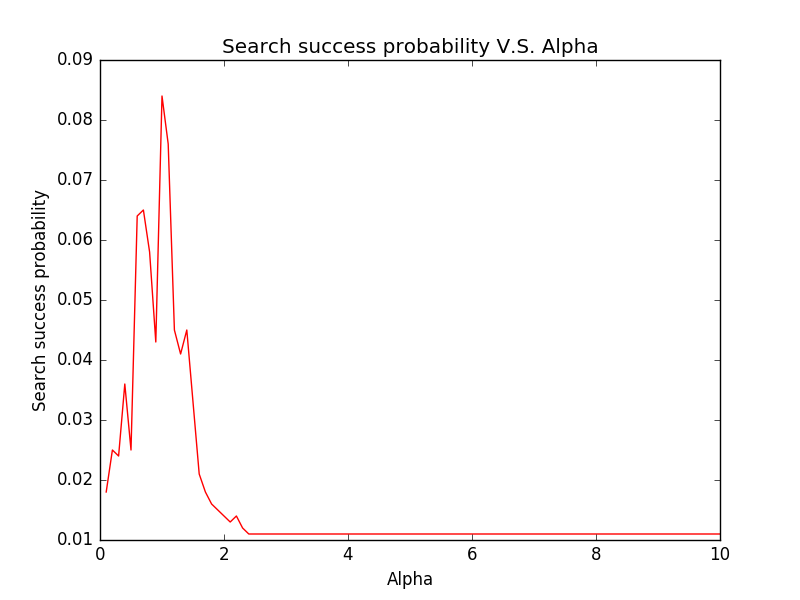
\includegraphics[width=\textwidth]{suc_s_prob.png}
  \caption{Search success probability V.S. Alpha}
  \label{fig:Search success probability V.S. Alpha}
 \end{subfigure}
 \begin{subfigure}{.5\textwidth}
   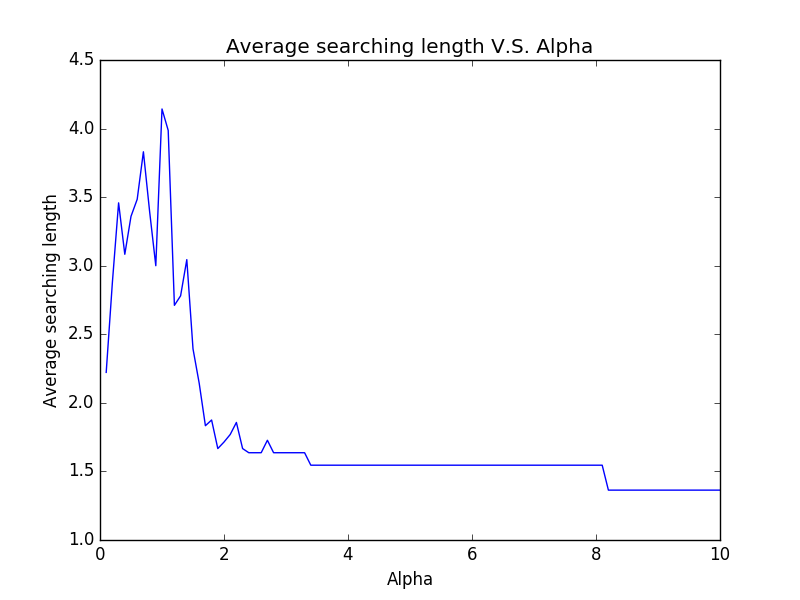
\includegraphics[width=\textwidth]{avg_s_len.png}
  \caption{Average searching length V.S. Alpha}
  \label{fig:Average searching length V.S. Alpha}
  \end{subfigure}
\end{figure}

As $\alpha$ goes up, we are making the graph to have more short edges and less long edges. \\
At first when $\alpha$ is small, we have too many long edges and too less short edges, the long edge enables us to travel quickly and get near to the target node but the lack of short edge limits our ability to actually arrive at the target. So we have relatively low search success probability. But if we can indeed find the target, we can do that pretty fast thanks to the abundant of long edges, so we have relatively low average search length.\\
Then as $\alpha$ grows, we begin to have enough short edges that help us to actually find the target, so we have rise in search success probability. But this is done at the expense of having less long edges so we may need to travel more steps in order to get to the target, this results in that we have longer average search length.\\
Then as $\alpha$ grows even bigger, we have almost only short edges. This makes us lack the ability to arrive at any of the nodes that are relatively far from us, which makes up a large proportion of the total nodes, therefore we have lower search success probability. However, if we are lucky enough to reach a target, it would be in the vicinity of our starting point and it costs small steps to get there, therefore we also have low average search length.


% Information sheet
% Fill out the information below (this should be the last page of your assignment)
\addinformationsheet
{\Large
\textbf{Your name:} \ Bowen Yao  % Put your name here
\\
\textbf{Email:}\ boweny@stanford.edu  % Put your e-mail here
\textbf{SUID:} \ 06129749  % Put your student ID here
\\*[2ex] 
}
Discussion Group: \ None   % List your study group here
\\
\vfill\vfill
I acknowledge and accept the Honor Code.\\*[3ex]
\bigskip
BY% Replace this line with your initials
\vfill





\end{document}
